\documentclass[a4j,twocolumn]{jsarticle}
\usepackage[dvipdfmx]{graphicx}
\usepackage{url}

\setlength{\textheight}{275mm}
\headheight 5mm
\topmargin -30mm
\textwidth 185mm
\oddsidemargin -15mm
\evensidemargin -15mm
\pagestyle{empty}


\begin{document}

\title{Rubygemsを用いたプログラミング言語Ruby学習の効率化}
\author{情報科学科 \hspace{5mm} 27015464 \hspace{5mm} 大津隆輝}
\date{}
\maketitle

\section{背景}
西谷研究室ではプログラミング言語Rubyを使用して,言語学習や卒業研究を行なっている.
つまり,3年生はRubyの習得が早ければ自分の研究の為の時間を確保できる.
しかし,個人で言語学習を行う際のハードルは高いものである\cite{Oshimi}.
その原因として,言語に対しての知識がない初心者にとって環境構築や学習の教材選びは非常に困難であることが要因の一つではないかと考えられる.環境構築なしで教材選びも必要ない言語学習サービスにはProgate\cite{Progate}やcodecademy\cite{codecademy}等があるが,環境構築という部分を排斥しているが故にそのサービス外での学習に一定の壁が生じているのではないかと考える.
\par
また,近年ではコードをGitで管理することで,チーム内でのコード編集の履歴をメンバーがそれぞれ確認することが出来るので,チームでの開発が管理しやすくなった\cite{GitDevelopment}.このような開発では他人の書いたコードを読み解き,それに適切な形で自分のコードを書き加える能力が必要となる.そう言った意味でも,近年の言語学習は動くだけのコードを書くのではなく言語が持つスタイルについてもきちんと学ぶ必要があると考える.
\par
そこで本研究では,環境構築の自動化に加え,Rubyの体系的な言語学習とプログラミングスタイルの学習ができるアプリケーションを開発し,Rubyを容易に学習できる環境を整え,実践的な学習を提供することで,個人のスキル向上の効率化を目指す.
\section{手法}
本研究ではGemアプリケーションruby\_learner\cite{RubyGems}を作成することで学習支援を行う.
このアプリケーションの主な機能はemacsを用いたRubyの学習(体系的な学習・実際の開発習慣の習得)・開発環境構築の自動化である.
上記の機能のうちRubyの学習には,テキストと課題の提供を行うことで使用者のインプット・アウトプットを通して記憶の定着を促す.
\par
学習の手順として,アプリ使用者にはテキストを読んでから課題に挑戦してもらう.
課題挑戦時に使用者の回答コードが適切なものであるかを2つのチェック項目から判断する(図\ref{fig:one}).
一つ目は,コードが期待される振る舞いをしているかである.
期待される振る舞いの確認とは課題の意図する通りに使用者の回答コードが動作しているかの確認である.
これはRSpecファイル\cite{rspec}と呼ばれるRuby向けのテストコードを記述するファイルを用いることで実装する.
このチェック項目を設けることで,本研究の先駆けとなったeditor\_learner\cite{editor_learner}とは違い,使用者の独創性を尊重するコードテストを行うことができる.
二つ目のチェック項目は,コードがRubyのプログラミングスタイルを遵守できているかの確認である.
%Rubyのプログラミングスタイルには
%・インデントは2スペース
%・クラス名はキャメルでそれ以外はスネーク
%・不要な改行がないか
%等が挙げられる.
これはrubyのプログラミングスタイルをチェックするGemアプリケーションRuboCop\cite{rubocop}を用いることで実装する.
このチェック項目を設けることで,使用者は自分のコード内に存在するプログラミングスタイルから外れている部分を確認することができる.
これら二つのチェック項目をクリアして課題の正解としている.

\begin{figure}[h]
\vspace{0\baselineskip}
\begin{center}
  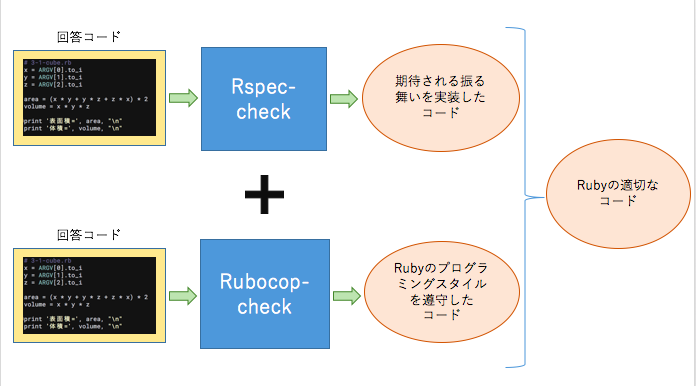
\includegraphics[width=70mm]{./rspec_rubocop.png}
  \caption{ruby\_learnerのrspecとrubocopを用いた2段階チェック構造.}
  \label{fig:one}
\end{center}
\end{figure}

環境構築の自動化は,本アプリ外でもアプリ内で行った環境でRubyの開発が行えるようにrubocop等のアプリケーションの自動インストールやemacsの設定ファイルの提供などを行う.

\section{予想される結果}
使用者は本アプリを通して,Rubyのプログラミングスタイルを遵守した上で期待される振る舞いをするコードの作成能力を習得する.また,その知識をアプリ外でも実戦で使える環境を手に入れることができる.上記の二つの効果により,使用者はアプリ外での言語学習も効率的に行えると考える.

\vspace{0.5\baselineskip}

{\small\setlength\baselineskip{10pt}    % 参考文献は小さめの文字で行間を詰めてある                                             
\begin{thebibliography}{9} 
\bibitem{Oshimi} 「Learning Style Inventoryを用いたプログラミング初学者のための教材レコメンドシステムの提案」押見太雄, (2017) p.1.
\bibitem{Progate} Progate. \url{https://prog-8.com/mypage}.
\bibitem{codecademy} codecademy. \url{https://www.codecademy.com/}.
\bibitem{GitDevelopment}  Git. \url{https://git-scm.com/book/ja/v2/}.
\bibitem{RubyGems} RubyGems. \url{https://rubygems.org}.
\bibitem{rspec} RSpec. \url{http://rspec.info/about/}.
\bibitem{editor_learner} editor\_learner 1.1.2, Souki Wada. \url{https://rubygems.org/gems/editor_learner/}.
\bibitem{rubocop} RuboCop. \url{http://batsov.com/rubocop/}.
\end{thebibliography}
}
\end{document}
